% LaTeX Template for a short article
%
% To use:
%
% Copy into a new file, replace all
% [BRACKETED UPPER CASE TEXT]
% with your own, then run the latex command on it.
% Use dvips to print the .dvi output
\documentclass[12pt]{article}
%These are packages that allow you to access LaTeX, like math symbols, fonts, colors, picture environments, etc.  There are many other packages available to do a variety of things.
\usepackage{graphicx}
\usepackage{pslatex}
\usepackage{amsmath}
\usepackage{amssymb}
\usepackage{color}
\usepackage{epsf}
\usepackage{tikz}
\usepackage{helvet}
\usepackage{physics}
\renewcommand{\familydefault}{\sfdefault}
\usepackage{hyperref}
\usepackage{subcaption}
\textheight9in \oddsidemargin-.5in \textwidth7in \topmargin-.5in

\def\Z{\mathbb Z}
\def\R{\mathbb R}
\def\C{\mathbb C}
\def\N{\mathbb N}
\def\Q{\mathbb Q}
\def\noi{\noindent}
% You may define a latex command of your own using the \def command.  Anything you type inside the {} will be executed in the text where you use the \contradiction command.  Below are a few other commands that I have defined.

\begin{document}

\title{Complex Analysis in Quantum Mechanics \\
Math 646 -- Final Project}
\author{Jonah Berggren, Thomas Gartman, Quinn Meier, and Kyle Turner}
\date{November 19, 2018}

\maketitle%This command inserts the title, author and date as defined above.

\begin{abstract}
Over the past century, quantum mechanics, the study of nature on the scale of subatomic particles, has evolved into the most accurate scientific theory of all time. All of this success wouldn't have been possible without the development of complex analysis and the novel mathematical ideas which have arisen from it. In this paper we shall provide a cursory overview of wave mechanics in the quantum world and explore some of the math describes it so elegantly. 
\end{abstract}


\section{Introduction}%this creates a section title 

Just as many mathematicians initially found the complex numbers an absurd notion, after being discovered in the process searching for roots of polynomials \cite{Needham}, there was a similar debate in quantum mechanics during its infancy. While complex numbers are frequently useful in the domain of classical mechanics and electrodynamics, they are not fundamentally necessary, as the variables corresponding to observable quantities are strictly real. This is makes sense as all measurements in physics result in real numbers \cite{MIT}. Despite this, complex numbers are \emph{essential} to quantum mechanics for reasons which can be seen by examining the general form of the Schr\"{o}dinger equation,
\begin{equation}
\boldsymbol{i}\hslash \frac{d}{dt} \ket{\psi(t)} = \Hat{H} \ket{\psi(t)}
\end{equation} 
which is solved by a wavefunction $\psi$ and takes the form of a partial differential equation when projected into an eigenbasis of some observable quantity such as position or momentum (where these two bases are related by a Fourier Transform) \cite{Shankar}. Since physics imposes that the action of the Hamiltonian ($\Hat{H}$), a linear operator that is numerically equivalent to energy, must be real, it follows that unless $\psi \in \C$ we will arrive at a contradiction. In other words, the wavefunction, which contains all of the information in a quantum system \cite{Ralston}, is necessarily complex-valued. These solutions to the the Schr\"{o}dinger equation often take the form of plane waves like \begin{equation}
\psi(\Bar{x},t) = Aexp(\frac{\boldsymbol{i}(\Bar{p}\cdot \Bar{x} - Et)}{\hslash})
\end{equation} 
which is an extremely powerful and concise representation of many physical phenomena \cite{Feynman}.   Since complex-valued variables are not observable, expressing the measurable quantities to associate with a given wavefunction led to fervid argument among physicists \cite{MIT}. Max Born proposed describing quantum systems with probability amplitudes $|\psi|^2 = \psi^*\psi$ which must satisfy unity i.e. $\int_{-\infty}^{\infty} \psi^*\psi d^3x = 1$ which is at the heart of the Copenhagen Interpretation of quantum mechanics. Other famous physicists like Albert Einstein and even Schr\"{o}dinger himself were deeply unsatisfied with this and search for a more accurate interpretation of quantum phenomena is still a subject of some inquiry \cite{Griffiths}
\section{Method}
The team decided to implement a numerical solution to the Schr\"{o}dinger equation in Mathematica. After performing some research, we found a Wolfram Demonstration that solved an extremely complex non-linear Schr\"{o}dinger equation for specific initial and boundary conditions released under a creative commons license \cite{nonLinearMath}. Using this as our primary example and lodestar, we set out on a mission to generate waveforms with the linear Schr\"{o}dinger equation in one dimension. These solutions represented two wave functions, represented as our boundary conditions in the code, interacting as they propagate through space and time.  After several hours of learning\footnote{The Mathematica Documentation as a whole was a lifesaver.} and failing, we were able to successfully create the 3D plots in Mathematica! Below is the waveform we were able to generate.
\begin{figure}
    \centering
    \hspace{-2cm}
    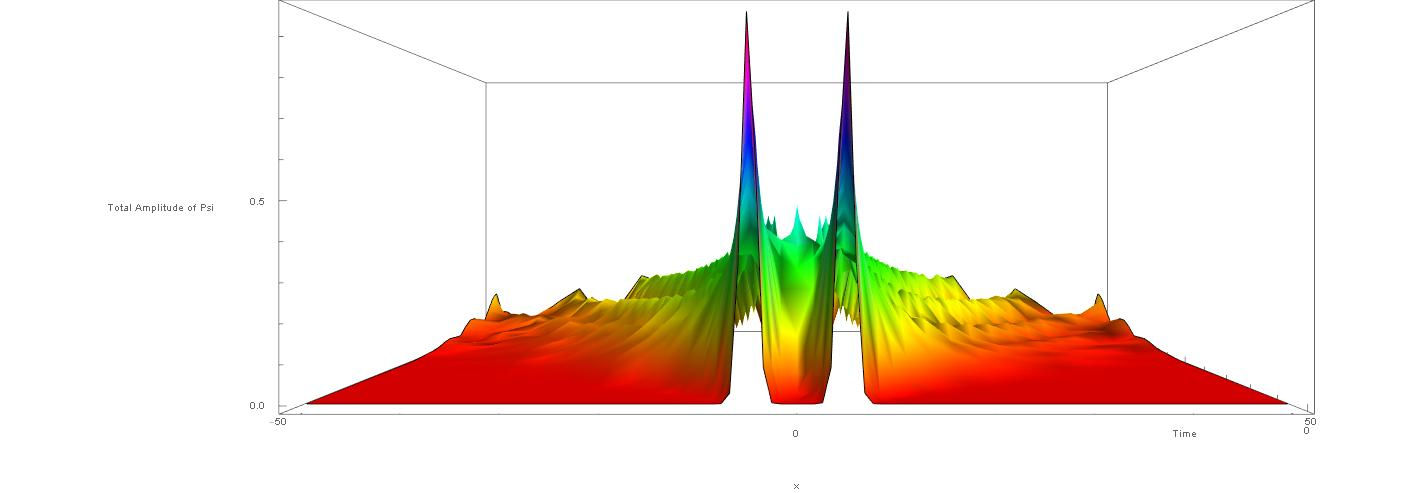
\includegraphics[width=350pt]{MATH_646_Project_Group_4/frontView.jpg}
    \caption{Magnitude peaks of the Waveform}
    \label{Peaksview}
\end{figure}

\begin{figure}
\centering
\begin{subfigure}{.5\textwidth}
  \centering
  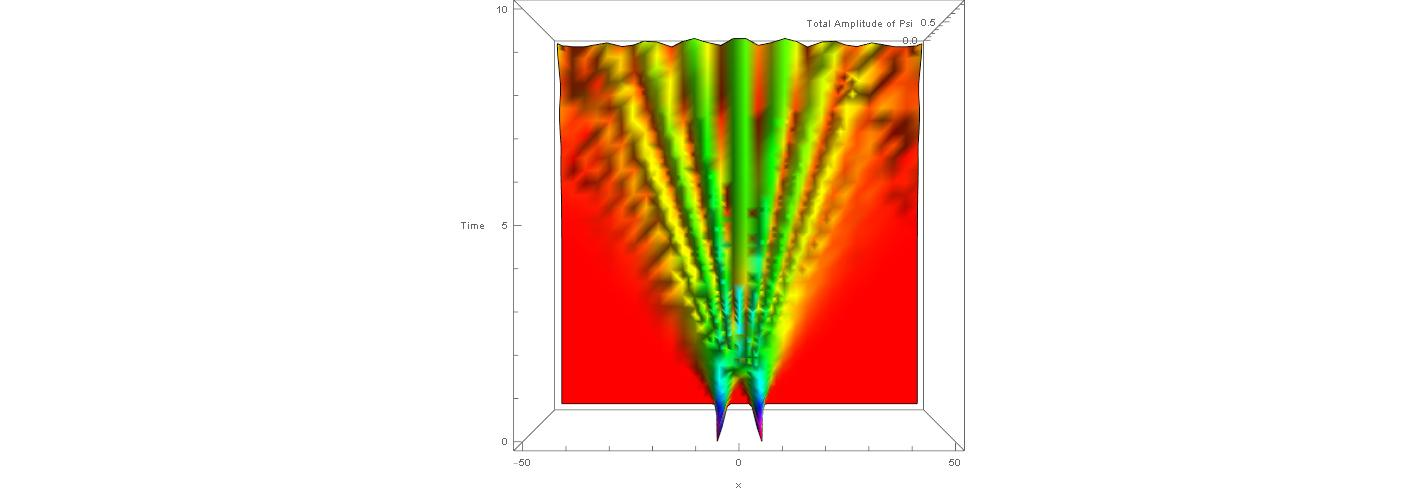
\includegraphics[width=1.1\textwidth]{MATH_646_Project_Group_4/topView.jpg}
  \caption{Top view}
  \label{Topview}
\end{subfigure}%
\begin{subfigure}{.5\textwidth}
  \centering
  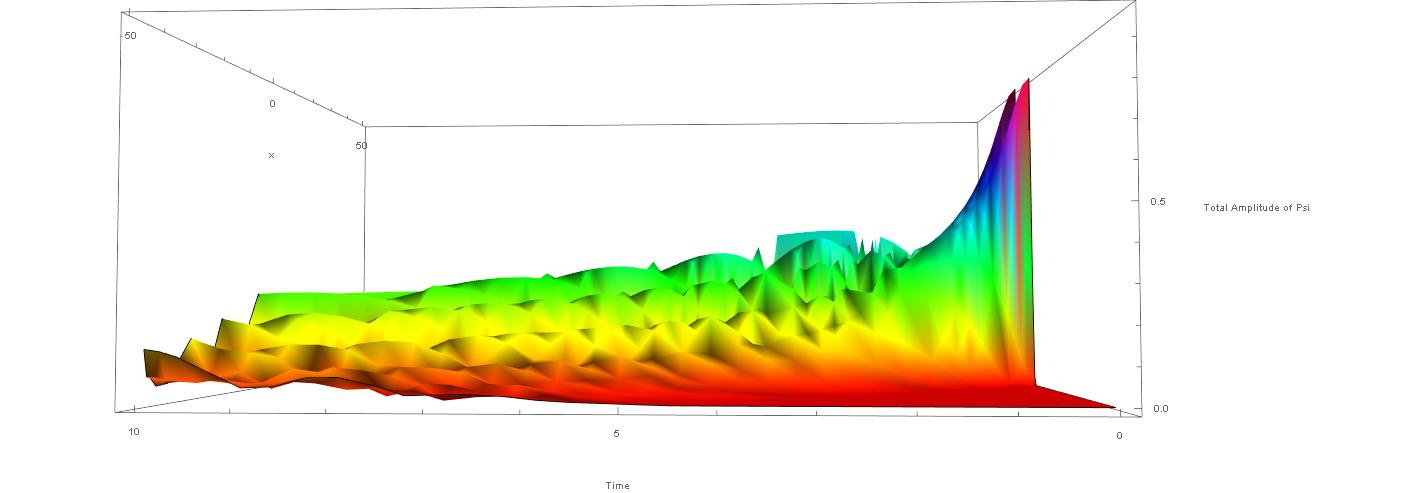
\includegraphics[width=1.1\textwidth]{MATH_646_Project_Group_4/sideView.jpg}
  \caption{Side view}
  \label{Sideview}
\end{subfigure}
\caption{Alternate viewpoints of the Waveform}
\label{Pictures}
\end{figure}

From Figure \ref{Peaksview}'s perspective, the bottom axis is position (x), the vertical axis is the total amplitude of probability amplitude of the wavefunction $|\psi(x,t)|^2 = \psi^*\psi$, and the axis into the page is time progression (t).

\section{ The Fabrication Process}
With the 3D plots in hand, now is the time to generate the 3D printed object!
\subsection{Creating the 3D Object}

\subsection{Novel Mathematical Properties}



\subsection{Strengths and Weaknesses of Model}

The limited number of dimensions in 3D is a severe limitation on the model and its 3D printout. Specifically, these waveforms are most interesting as they move through time. Without being able to print many of these waveforms, one of each time step, we lose the fluidity of other models freely available.\\\\
However, spending time examining printed models of a snapshot in time allows for a fuller examination of how the waveform is impacted specifically on position. This includes how the imaginary and real parts of the waveform interact to form a cohesive system. Luckily, this confirms that the waveform probability directly depends on position, which conforms to quantum mechanical theory laid out in Ralston and Shankar \cite{Ralston} \cite{Shankar}. The 3D printed model also has pedagogical value as a visualization of the usually arcane graphs provided in introductory physics courses like \emph{PHSX 313: General Physics 3} at the University of Kansas.

\section{Conclusions - Future Work}

Overall, we are pleased with how the 3D model turned out! Modeling linear (and non-linear) partial differential equations appears to be closely tied to complex analysis and an understanding of the former requires strong skills in the latter. \\\\
Despite us being able to generate a pair of free particles and their interactions with each other, we would enjoy continuing to explore more of these kinds of models. One of the more interesting aspects of development would be to set up a maze or other complex structural system of high potentials to see how a particle might propagate through such a complex potential. Seeing this in a 3D-model would help build intuition for how these kinds of interactions unfold. Additionally, we could explore models with 
\newpage

\begin{thebibliography}{9999}
\bibitem{Needham} Tristan Needham, Visual Complex Analysis, Oxford University Press, 1997.
\bibitem{MIT} B. Zwiebach, Overview of Quantum Mechanics, MIT OpenCourseWare, 2016. Accessed: 13/11/18 \url{https://ocw.mit.edu/courses/physics/8-04-quantum-physics-i-spring-2016/lecture-notes/MIT8_04S16_LecNotes1.pdf}.
\bibitem{Shankar} R. Shankar, Principles of Quantum Mechanics 2nd Edition, Plenum, 1994. 
\bibitem{Ralston} John P. Ralston, Understanding Quantum Mechanics, Monte Carlo, 2017.
\bibitem{Feynman} Richard Feynman Et Al., The Feynman Lectures on Physics, Volume III, CIT, 1965.
\bibitem{Griffiths} David J. Griffiths, Introduction to Quantum Mechanics, 2nd Edition, Pearson, 2004.
\bibitem{nonLinearMath} Enrique Zeleny, Solution of a Nonlinear Schr\"{o}dinger Equation, Wolfram Demonstrations, 2012. Accessed: 11/11/18 \url{http://demonstrations.wolfram.com/SolutionOfANonlinearSchroedingerEquation/}.


\end{thebibliography}

\section{Group Members and Contributions}
\begin{enumerate}
\item {\em Jonah Berggren} \\
\underline{Contribution}: Used knowledge of Mathematica to help graph the function, and checked for mathematical consistency of the project. Wrote and edited portions of the LaTeX report document.\\
\item {\em Thomas Gartman} \\
\underline{Contribution}: Used knowledge of PDEs and physics to assist in modeling the waveforms. Helped generate the 3D object files. Enforced version control on the project in the form of Github. Wrote a majority of the LaTeX report document. \\
\item {\em Quinn Meier} \\
\underline{Contribution}: Had the knowledge of Quantum Mechanics and Schr\"{o}dinger Equations in particular. Quinn used his Mathematica jujitsu to generate the 3D plots. Wrote and edited portions of the LaTeX report document. \\
\item {\em Kyle Turner} \\
\underline{Contribution}: Helped to graph and synthesize Mathematica code for the function and converted the finished program to the proper format ready to be printed. Wrote and edited portions of the LaTeX report document.   \\

\end{enumerate}


\appendix
\section{Codebase}\label{code}

Below are the scripts we used to generate the 3D object. The code can also be found at our GitHub page: \url{https://github.com/QMeier/MATH_646_Project_Group_4}.


\end{document}

